\chapter{Data-driven decision making}{“The knowledge domain is a very important aspect of what we are looking for.”}



Chapter \ref{chap_InformationFramework} introduced the entities and the metrics of a supply chain system. This book deals with these entities from a system analysis perspective (see section \ref{secSupplyChainTaxonomy}), i.e. considering the design and control alternatives to manage the operations of a distribution network, a storage system, or a production plant. These problems have been mostly addressed by decision science. The following chapters aim at identifying boundaries between decision science, and data science in the system analysis of a supply chain system. It will be remarked, as well, where data science is ready to compete with decision science to address a decision problem.\par

It is crucial to consider the knowledge domain of supply chain systems to do this job. While decision science has the ability to model each problem precisely, with instance-tailored boundaries and objective functions, we aim at designing a high-level classification of supply chain system problems. We identify patterns among similar decision problems encountered in different supply chain systems whose entities are defined by the ontology in \ref{secOntology}. Each decision pattern is identified by an id used in the following chapter as reference.\par

The following section introduces a glossary of data and information to understand the meaning of these words correctly; the classification of the decision patterns; a method to choose the right analytical technique to address a supply chain system problem, given its data, and its decision pattern; a summary of the main contributions of this book.

\section{Data Glossary}

Since this book deals with data, it is important to remark some crucial aspects. The traditional engineering modelling approach is based on intuition. The researcher observes a logistic phenomenon, makes assumptions, build a model, and fit the empirical data to the model. The data-driven approach is profoundly different since it collects data and different models fit the data, identifying the model with the best fit.\par

Our data collection activities involve multiple entities since we use a top-view perspective, looking at the system analysis. For this reason, we may have multiple data sources with redundant information, different synchronism, different granularities, different data protocols. Table \ref{tab_data_glossary} introduces the glossary explaining all these elements.

% INSERT tab_data_glossary
\begin{figure}[hbt!]
\centering
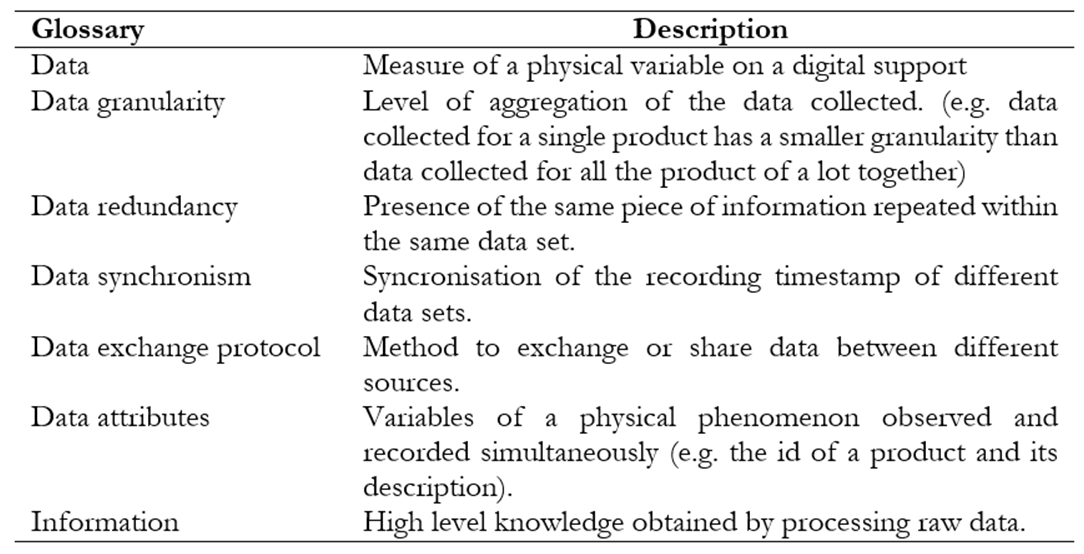
\includegraphics[width=1\textwidth]{SectionIntroduction/dataDrivenDecisions_fig/tab_data_glossary.png}
\captionsetup{type=table}
\caption{Glossary of data-related terms.}
\label{tab_data_glossary}
\end{figure}

\section{Decision patterns} \label{secDecisionPatterns}
Entities are connected with relevant strategic and control issues that must be addressed to properly organise the operations of a warehouse, production plant, or distribution system. The literature defines these issues as problems, using mathematical models. We organise these problems by introducing an original classification, with ten classes. Each class is addressable by the same branch of analytics (descriptive, explorative, predictive, or prescriptive), depending on the type of problem. 

\paragraph{Family problems (P1)}
This class of problems aims at defining homogeneous clusters of parts, to simplify the organisation of operations. Issues belonging to this class concern definitions of product families with the same production cycle (i.e. the route), and definitions of classes of stock-keeping units (SKUs) with similar characteristics (e.g. weight and volume). Descriptive and explorative analytics offer tools to assess the features of parts and to produce clusters. 

\paragraph{(Technology) Assignment problems (P2)}
This class of problems solves the assignment of parts to resources and vehicles from a high-level strategic perspective. Some examples are the assignment of SKUs to storage locations, the assignment of points of demand to trucks or the identification of the families of product to be processed by a resource (e.g. a production line or an FMS). The best configuration is found by the evaluation of every single alternative (prescriptive methodologies) or the definition of homogeneous clusters by an explorative technique.\par

Problems involving the definition of adequate technology for production nodes belong to this class and can be addressed using the same rationale. The definition of the storage system technology (storage rack with/without forward-reserve, floor stack, automated storage technology) and the identification of the level of automation in a production plant are examples of these problems. The technological choice in a distribution network (i.e. truck/rail/water/air) is neglected since it is imposed by the existent infrastructure or by political choices falling outside the domain of this research. The choice of the vehicle is solved in an operational environment with synchromodality i.e. when multiple transportation options exist for the same transportation unit (e.g. a pallet on a barge or a truck).

\paragraph{Flow problems (P3)}
This class of problems identifies how processing nodes are connected. They only exist for warehouse and production nodes since the design of the distribution infrastructure belongs to transportation science, and it is outside the domain of this research. The definition of the rationale to travel within storage racks (i.e. return or traversal policy) and the identification of paths for conveyors and forklifts in a production plant are examples of these problems. As for technology assignment problem, flow problems need prescriptive tools to identify efficient handling solutions.

\paragraph{Mechanical plant and equipment design (P4)}
This class of problems addresses engineering issues, such as the design of power plants, thermal plants, mechanical plants, lighting systems, air conditioning systems, and/or the physical designs of workbenches, material slots, and ergonomics. All these activities usually have poor historical data, and it is difficult to structure a series of previous observations of data addressing the same problem. For this reason, prescriptive models often address these problems by relying on an engineering model describing the dynamics or thermodynamics of the system.

\paragraph{Power problems (P5)}
This class of problems identifies the amount of power required for a specific resource $j$, and defines its capacity $C_j$. The storage allocation and design of areas for inbound/outbound operations are examples of power problems in a storage system. The design of the frequency of a route and service time windows at a terminal are power problems in a distribution network; the definition of the number of machines of the same type is a version of this problem in a production node. Prescriptive tools allow for solving these problems.

\paragraph{Placement problems (P6)}
A placement problem defines the identification of the proper disposition of entities (e.g. resources or set of parts) on the plant layout of a production system or storage system. Examples include the definition of a plant layout or location of a facility, the assignment and placement of SKUs to warehouse zones, the definition of the location of the facilities of a distribution network (location-allocation problem). Prescriptive and explorative techniques address these problems by clustering parts with similar behaviour (e.g. placing the same resources close to each other). 

\paragraph{Dispatching rules (P7)}
This class of problems provides rules for organising operations among the many possibilities and uncertainties that may occur in practice. The definitions of the shipping priority for transportation units and the picking policy (e.g. batching, sorting, pick and pack, single-order picking, cross-dock) for SKUs are examples of dispatching rules. In a production environment, the choice between a pull or a push policy is another dispatching rule. Dispatching rules affect the level of the work in process, size of the lots, and rationale for satisfying the market demand (i.e. pull/push). The definition of these rules requires a prescriptive model.

\paragraph{Performance assessment (P8)}
This class of problem is deliberately descriptive. It aims to describe the system $G$, its entities (i.e. parts, resources and vehicles), and its processes (i.e. jobs and routes). Data science offers tools to approach this type of problem, as the results are obtained exclusively using descriptive and explorative tools for evaluating the log data from a storage system, production system, or distribution network.

\paragraph{Workload predictions (P9)}
This class of problems aims at forecasting the values of relevant variables regarding a product or a process in the future. The predictions are influenced by market demand. Hence, predictions consider the number of parts (e.g. SKUs, containers, or products) which will be processed by a system $G$ in the near future. The estimate of the number of parts leads to the prediction of other relevant process variables (e.g. the speed of a machine, or number of operators required to perform activities).

\paragraph{Operations management (P10)}
This class of problems prescribes how to act within given circumstances to perform operations. This problem always involves a prescription, e.g. the definition of a sequence of products to process on a machine (job scheduling), or the sequence of locations to visit from a truck in a distribution system or a forklift in a warehouse system. Prescription tools can approach these problems when the input data are consistent and compliant with their hypotheses. In particular situations, predictive and explorative tools may be used to address the problem as well. For example, when processing a single part to assign to a resource in an online version of the problem (e.g. a last-minute order to assign to a production machine), a prediction or clustering model based on robust data can solve the assignment, given the current state of the system $G$.

\section{Decision trees}
Once the class of analytics (i.e. descriptive, explorative, predictive, or prescriptive) for solving a problem has been defined, it is necessary to identify the technique for obtaining a solution. Different methodological paths exist to solve a problem $P$, depending on:

\begin{enumerate}
    \item the need to set up decision variables D to solve the problem (e.g. in prescriptive analytics);
	\item the availability of measurements on previous realisations of the solution;
	\item the completeness and the accuracy of the realisation dataset; and
	\item the knowledge on the boundary conditions of $X$.

\end{enumerate}

We introduce three original decision trees to identify these paths, and to guide the decision-maker in the definition of the proper technique to address a problem. Decision trees focus on descriptive, predictive, and prescriptive analytics, whereas exploratory analytics appears in some branches of the other trees.

\subsubsection{Descriptive decision tree}
This tree aims at the description of a variable $y$ as a random variable; $y$ is usually a KPI metric, and there are no decision variables $D$ to set up. Sometimes, it is impossible to directly measure a variable on-field (e.g. often when $y$ is a cost). In these cases, it is necessary to link the value of $y$ with a kinematic model $y=f(X)$, based on a set of measurable variables $X$ that are inputs of a motion equation $f$. The variables $X$ usually describe the movements of a logistical process (e.g. the path travelled by a truck on a road or by a forklift within a plant). Once $f$ is defined, a numerical simulation (e.g. Monte Carlo simulation) allows for investigating the behaviour of $y$, depending on the distribution of $X$ and on the tuning parameters of the kinematic model. When $y$ is measurable but the dataset presents different data sources with different levels of accuracy, Bayesian statistics can be used to infer the properties of $y$ by leveraging its estimate and considering the reliability of each input data source. Otherwise, the inferential statistic is appropriate when the data are from a single source, and there are no measurements $Y$ of other variables linked to $y$. When a dataset $Y$ containing observations of a set of variables connected to $y$ is available, explorative analytics (i.e. clustering) is suitable for investigating the correlations between the variables and improving the knowledge of the decision maker regarding the important variables affecting the process. Figure \ref{fig_describe_tree} introduces the descriptive decision tree, and illustrates the decision steps identified above.

% INSERT fig_describe_tree
\begin{landscape}
\thispagestyle{empty}
\begin{figure}[hbt!]
\centering
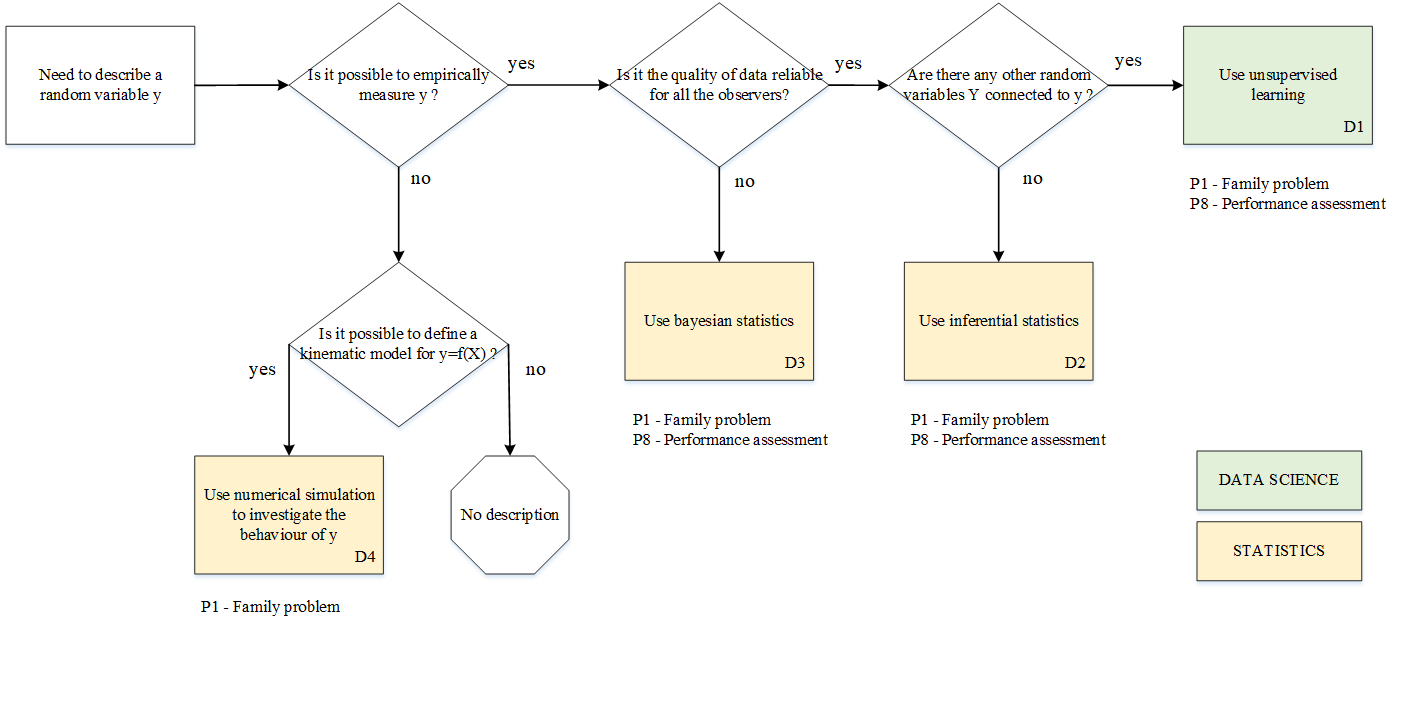
\includegraphics[width=1.5\textwidth]{SectionIntroduction/dataDrivenDecisions_fig/fig_describe_tree.png}
\captionsetup{type=figure}
\caption{Decision tree for descriptive purposes.}
\label{fig_describe_tree}
\vfill
\end{figure}
\end{landscape}




\subsubsection{Predictive decision tree}

This tree aims at forecasting future realisations of a variable $y$, given its description as a random variable. For this reason, there are no variables $D$ to set up (except for the hyperparameters of some forecasting models). The ability to empirically measure the variable $y$ is a key branch of the decision tree. If the variable cannot be measured directly (e.g. the inventory position of a truck while travelling), the only other option is to define a kinematic model to estimate its value (e.g. estimating the inventory using loading and unloading records). Without a kinematic model and/or a direct measurement, it is impossible to make predictions. When the variable can be measured but the measures are incomplete (e.g. a small subset of the dataset), explorative clustering techniques can be used to extend the properties measured for the small sample to the entire population $\widetilde{y}$ (e.g. from a subset of parts to an entire product family). In this case, it is necessary to have a validation dataset $\hat{y}$ associated with the values of $\widetilde{y}$. If a validation dataset is not available, the kinematic model remains the sole alternative for obtaining an estimate. Otherwise, it is possible to set a prediction model. When there are no other variables $Y$ associated with $y$, time-series forecasting (e.g. decomposition, Fourier analysis, autoregressive integrated moving average (ARIMA) models) can be used to make predictions. When a dataset of variables $Y$ associated with $y$ is available, supervised machine learning models can lead to more accurate predictions. Figure \ref{fig_predict_tree} illustrates the decision tree, along with the decision steps identified above.

% INSERT fig_predict_tree
\begin{landscape}
\thispagestyle{empty}
\begin{figure}[hbt!]
\centering
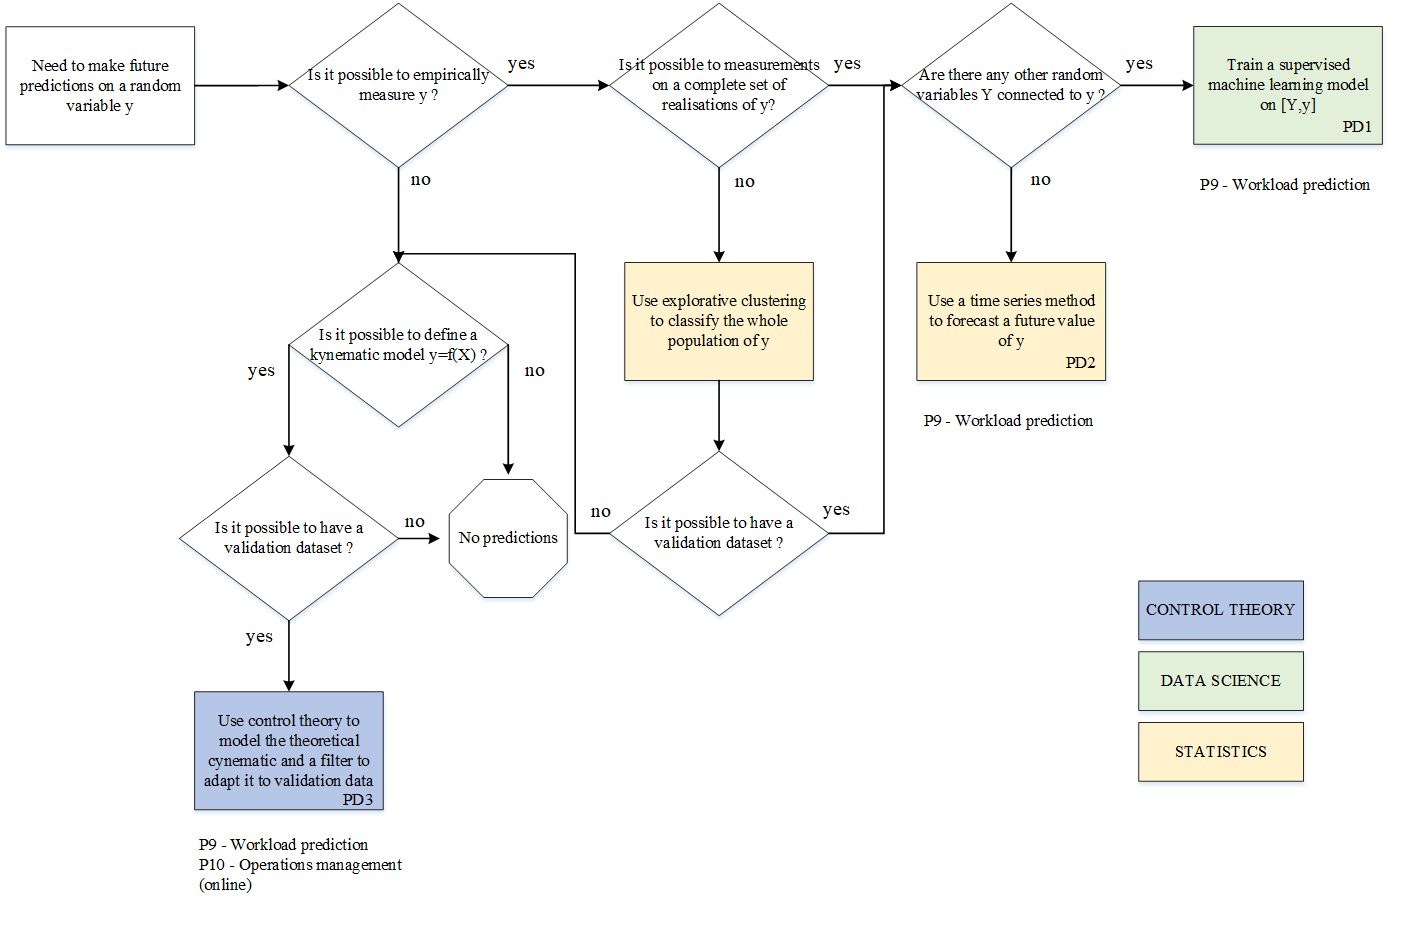
\includegraphics[width=1.5\textwidth]{SectionIntroduction/dataDrivenDecisions_fig/fig_predict_tree.png}
\captionsetup{type=figure}
\caption{Decision tree for predictive purpose.}
\label{fig_predict_tree}
\vfill
\end{figure}
\end{landscape}

\subsubsection{Prescriptive decision tree} \label{secPrescriptiveDecisionTree}
When addressing prescription problems, it is necessary to identify a set of decision variables $D$, such that an objective on $y$ can be reached (e.g. a cost can be minimised). As for the previous trees, when $y$ cannot be directly measured, it is necessary to define a kinematic model $y=f(D)$. If no validation dataset $\hat{y}$ is available, there is no scientific way to set $D$. Otherwise, control theory can help to adapt the kinematic model to realisations in the real world. The optimal solution is obtained by using mathematical minimisation (e.g. derivatives) on the motion equations of the system. When measurements are available on a subset of realisations of $y$, unsupervised clustering is used to extend the properties of the observed dataset with a clustering function $y=g(D)$. If the problem is an assignment problem, the clustering boundaries $g$ may be sufficient to solve the problem (e.g. assignment of parts to processing nodes); otherwise, it is necessary to enumerate all of the alternatives and to select the best one. When a dataset with observations for all of the entities is available and it is possible to define a feasibility region for any value of $y$, optimisation should be used. Figure \ref{fig_prescribe_tree} presents the decision tree, along with the decision steps identified above.

% INSERT fig_prescribe_tree
\begin{landscape}
\thispagestyle{empty}
\begin{figure}[hbt!]
\centering
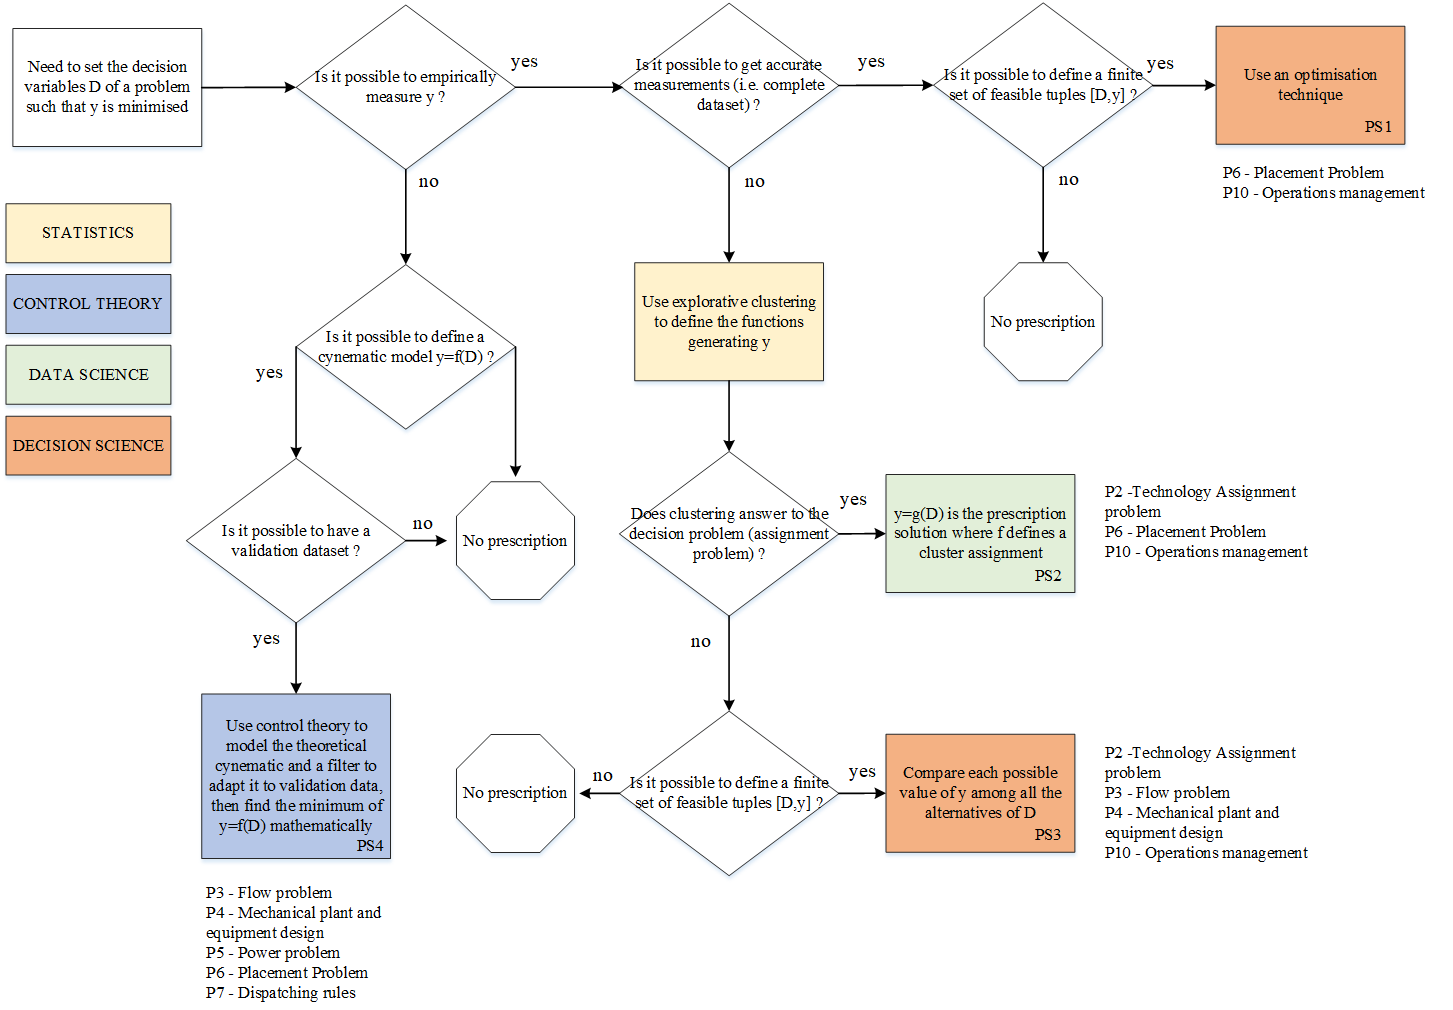
\includegraphics[width=1.5\textwidth]{SectionIntroduction/dataDrivenDecisions_fig/fig_prescribe_tree.png}
\captionsetup{type=figure}
\caption{Decision tree for prescriptive purpose.}
\label{fig_prescribe_tree}
\vfill
\end{figure}
\end{landscape}



The resulting classification of problems, analytics, and solving techniques is introduced in Table \ref{tab_problem_classification}. Each row of the table refers to a problem within its system domain (i.e. warehouse/production plant/distribution system). It identifies the type of decision (design or control) and the entities involved (e.g. part, vehicle). The right side of the table describes the classes of analytics that address the problem, and the methodologies for obtaining a solution (according to the labels used in the decision trees). For example, the first row of the table addresses the family problem (P1) in warehousing systems. This is a design decision involving the definitions of clusters of SKUs. SKUs are, then, the entities involved in being modelled as parts in the ontology. The problem is addressable by using descriptive or explorative methodologies, labelled as D1, D2, and D3 in the decision trees.


% INSERT tab_problem_classification
\begin{landscape}
\thispagestyle{empty}
\begin{figure}[hbt!]
\centering
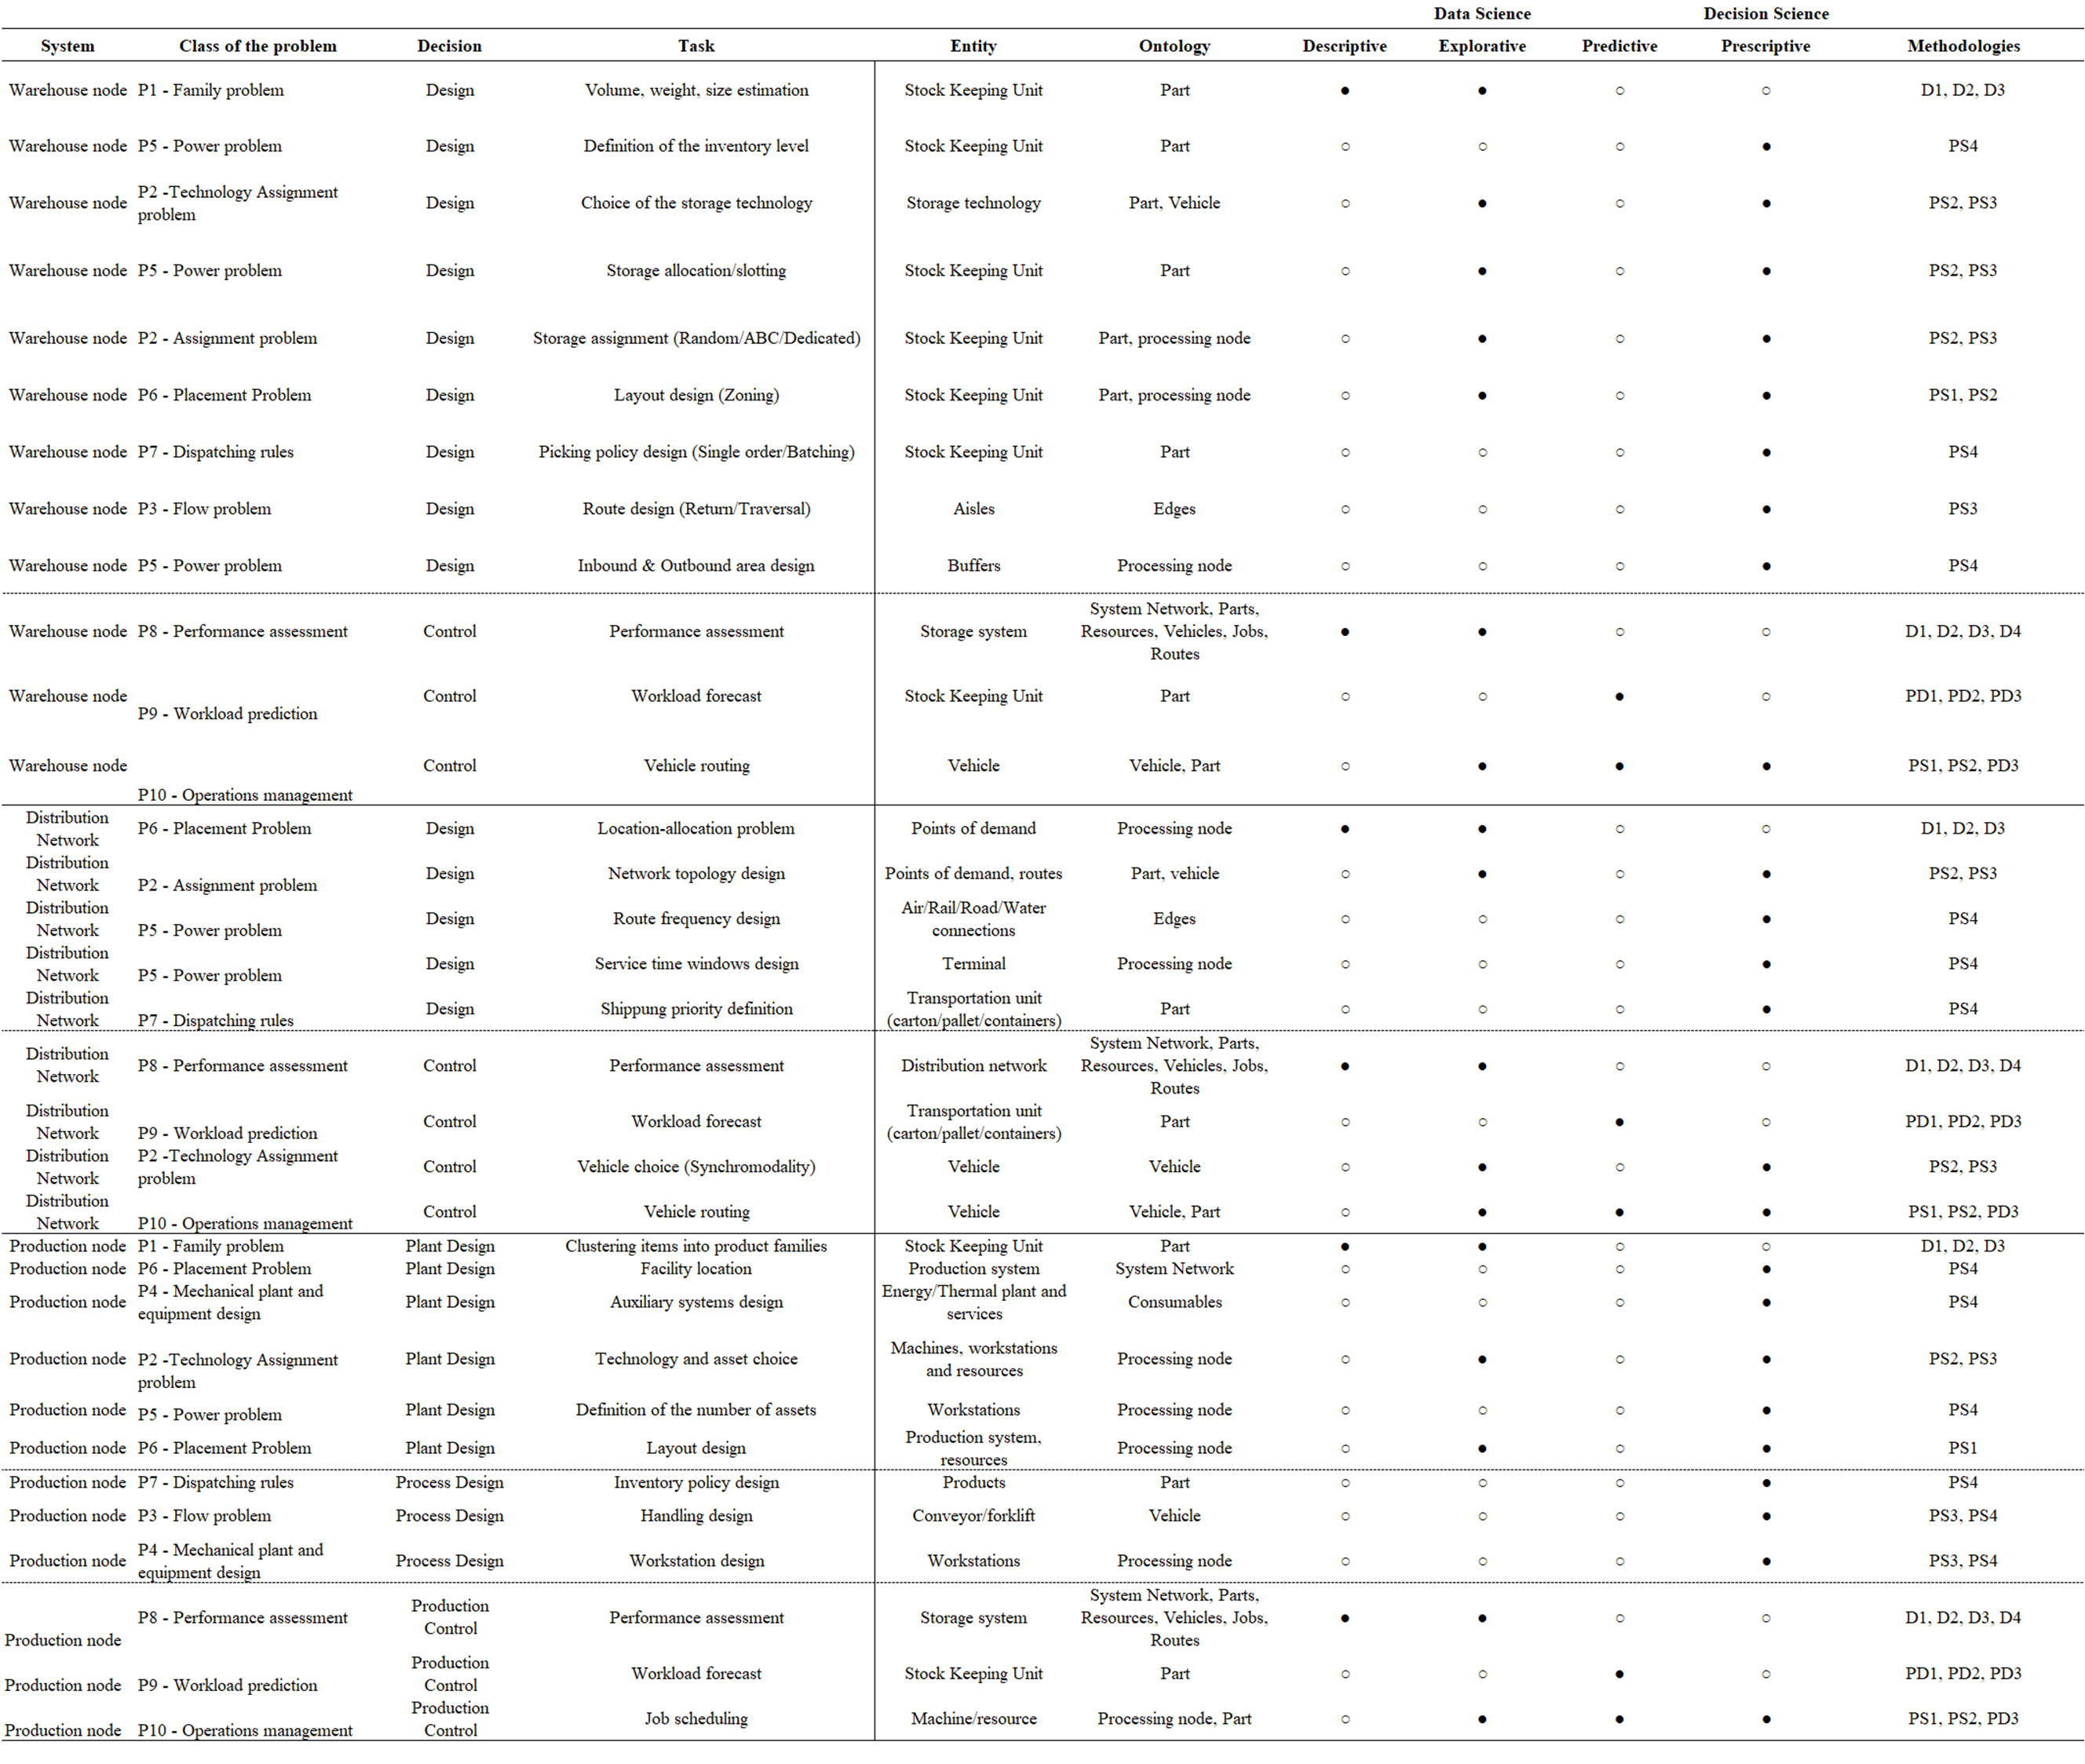
\includegraphics[width=1.3\textwidth]{SectionIntroduction/dataDrivenDecisions_fig/tab_problem_classification.png}
\captionsetup{type=table}
\caption{Definition of the problems for warehouse nodes, production nodes and distribution networks.}
\label{tab_problem_classification}
\vfill
\end{figure}
\end{landscape}

\section{Main contributions of this book}
Chapter \ref{chap_InformationFramework}, and the previous paragraph of this chapter, introduced a new method to structure data, and precise pattern to identify the analytical approach to solve a problem. The remainder of this book shows how to apply these elements to distribution networks, storage systems, and production plants.\par

In particular, we focus on the data-driven models presented in part II to show how to learn information from a dataset; while part III, IV, and V shows what information can be learnt from logistics and operational data.\par

We explore the role of data in logistics and operations research. The research, according to the first three paradigms, involves the design of a model and the optimisation of the modelled system using the models’ parameters. Here we use the fourth science paradigm; for this reason, the solely modelling activity involves the definition of consistency rues between data (i.e. the information framework introduced in chapter \ref{chap_InformationFramework}). For this reason, each of the following sections proposes relational, and non-relational data structures to host data from a specific industrial domain (i.e. warehousing, transportation and production). We will show that, if data are stored correctly, it is possible to define consistency rules to get the highest information even when the input data is incomplete. \par

Another important contribution regards the way we do research. Researchers must do experiments. Doing experiments at a system level is hard since it is impossible to build a lab containing a globally distributed supply chain. For this reason, we create virtual environments using digital twins of the entities of a supply chain. Then, we do experiments on these virtual entities. Data define the entities while scripts of code do the experiments on these entities. Our research becomes reproducible since the scripts can be run many times with different input data supporting the generalisation of our research. These scripts implement the analytics, that is the technology we want to explore and test in this research. There are two groups of scripts implemented within the virtual laboratory: general-purpose, and problem-oriented scripts.\par

General-purpose scripts implement general-purpose methods, i.e. pieces of code based on data-driven approaches that are not necessarily linked to the field of logistics and operation. All the methods illustrated in part II belong to this class of scripts.\par

Problem-oriented scripts find the solution of a problem by using a decision-pattern illustrated in \ref{secDecisionPatterns}, and may combine many general-purpose scripts. These methods are presented in part III, IV, V. \par

Another type of script manages the flow of data from the industrial data sources to the other type of scripts. Figure \ref{fig_data_flow} illustrates the flow of data. 

% INSERT fig_data_flow
\begin{figure}[hbt!]
\centering
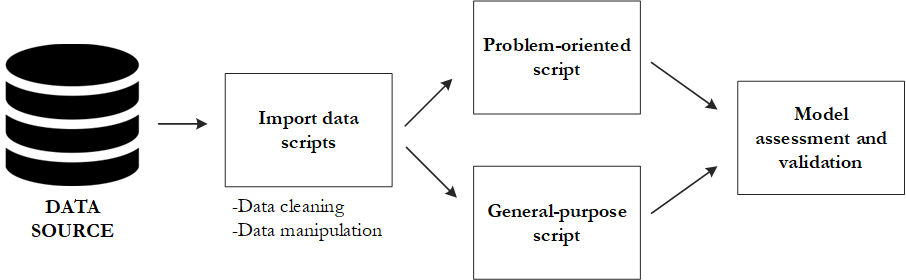
\includegraphics[width=1\textwidth]{SectionIntroduction/dataDrivenDecisions_fig/fig_data_flow.png}
\captionsetup{type=figure}
\caption{Data flow between scripts.}
\label{fig_data_flow}
\end{figure}

To support the research community in the field of supply chain systems with robust methods, and data structure, problem-oriented and general-purpose scripts are written using python, the most used programming language nowadays, and distributed with an open-source licence.\footnote{The package logproj contains general-purpose, and problem-oriented scripts \href{https://github.com/aletuf93/logproj}{here}.}

From a research perspective, we can state several research questions addressed by the contents of this book.

\textit{RQ1: Which data are needed to solve a problem in the field of logistics and operations?}\bigskip

\textit{RQ2: how to collect, organise, preprocess and manipulate this data?}\bigskip

\textit{RQ3: which method should be used to address an issue in the field of logistics and operations?}\bigskip

\textit{RQ4:  when the data-driven approach is recommendable to address a problem in the field of logistics and operations?}\bigskip

The remainder of this book  is organised as follows. Part II introduces and clarifies all the math, statistics and the basic models which will be applied in this book. Part III, IV and V are dedicated to a logistic system, i.e. storage nodes, distribution networks, and production plants. Each part has a similar structure illustrating:
\begin{itemize}
    \item The design of a diagnostic model to assess the entities and the metrics of a logistics system;
    \item The design of a relational data structure to store planned and actual logistics/operations data;
    \item The design of a non-relational data structure to store planned and actual logistics/operations data;
    \item Model-driven methods to address control issues of the logistic system;
    \item Data-driven methods to address control issues of the logistic system;
    \item Model-driven methods to address design issues of the logistic system;
    \item Data-driven methods to address design issues of the logistic system.
\end{itemize}






%\clearpage
%\bibliographystyle{ieeetr}
%\bibliography{SectionIntroduction/informationFramework_ref}